\documentclass[10pt,twocolumn]{article}

\usepackage{amsmath}						%math
\setlength{\columnsep}{0.5cm} 				%column separation
\usepackage{blindtext} 						%randomized text
\usepackage[english]{babel}					%languages
\usepackage{sansmathfonts}					%font selection
\usepackage[T1]{fontenc}					%font application
\renewcommand*\familydefault{\sfdefault}	%apply font to whole document
\usepackage{graphicx}						%image file insertion
\usepackage{float}							%figure alignment
\usepackage{paralist}						%list manipulation
\usepackage[margin = 0.75in]{geometry}		%custom margins
\usepackage{tabularx}						%custom width tables
\usepackage{hyperref}						%hyperlink setup
\usepackage{comment} 						%comment out blocks
\usepackage{subcaption}						%sub figures
\hypersetup
{
    colorlinks=true,
    linkcolor=blue,
    filecolor=magenta,      
    urlcolor=cyan
}
\usepackage{titlesec}									%custom title sizes
%\titleformat*{\section}{\Large\bfseries}
%\titleformat*{\subsection}{\large\bfseries}
%\titleformat*{\subsubsection}{\normalsize\bfseries}
%\titleformat*{\paragraph}{\small\bfseries}
%\titleformat*{\subparagraph}{\small\bfseries}
%\titlespacing*{\section}								%custom title spacing
%{0pt}{5pt}{5pt}
%\titlespacing*{\subsection}
%{0pt}{5pt}{5pt}
\setcounter{secnumdepth}{0}								%remove title numbering

%custom commands below
%%%

\begin{document}

\title{\huge{\textbf{Astable ICM7555 PCB}}}
\author{Raj Mudhar}
\date{May, 2021}
\maketitle
%\tableofcontents

\section{Description}

This mini project is meant to be an introduction to PCB design. It follows the tutorial provided by Contextual Electronics, which briefly covers how to convert a schematic into a PCB, specifically with surface mount components. This project is not meant to be complex, but rather gives an insight into the procedure of design $\rightarrow$ schematic $\rightarrow$ modelling $\rightarrow$ assembly. This includes IPC standards, although non-trivial for this prototype, how to effectively use component data sheets, the physical structure of a PCB, and the design practices that are used most often.

\section{Implementation}

During the design process, the following modifications were made:
\begin{compactitem}
  \item The addition of a switch  to cut-off the battery.
  \item Larger SMD components (1206) to give some additional error room when soldering.
  \item Custom libraries for the battery holder and switch.
\end{compactitem}

\subsection{Theory}

The CMOS 7555 timer was chosen due to its improved voltage range over the standard bipolar NE/SE555 timer, which allows a coin cell battery to be used. In fact, it is the exact equivalent to the NE/SE555  for most applications, especially as an astable multivibrator. The internal functional diagram shown in Figure \ref{fig1} includes two comparators, an SR latch, and an NMOS discharge transistor. The astable configuration shown in Figure \ref{fig2} can be described using the functional diagram shown in Figure \ref{fig2}, where pins 2 ($ \overline{\mbox{TRIGGER}}$) and 6 (THRESHOLD) control the state of the comparators.

Regardless of the values of resistors ${\mbox{R}}_{\mbox{A}}$ and ${\mbox{R}}_{\mbox{B}}$, the initial state at pin 3 is logic high (H), as the capacitor is held discharged by the internal NMOS discharge transistor. When the voltage across the capacitor voltage begins to increase, it reaches a value that is ${\mbox{2/3V}}_{\mbox{DD}}$+, which sets comparator A to output H. As a result, the SR latch is reset and the output is logic low (L). At this point, the NMOS transistor gate terminal is H, which allows the current to discharge from the capacitor through ${\mbox{R}}_{\mbox{B}}$ to ground. During this phase, the voltage on the capacitor drops below ${\mbox{1/3V}}_{\mbox{DD}}$, which sets the SR latch to output H, and turns the discharge transistor off. The capacitor begins to charge again and follows the same self triggering multivibrator effect. The waveform of the capacitor and output voltage can be seen in Figure \ref{fig3}.

\begin{figure}[H]
	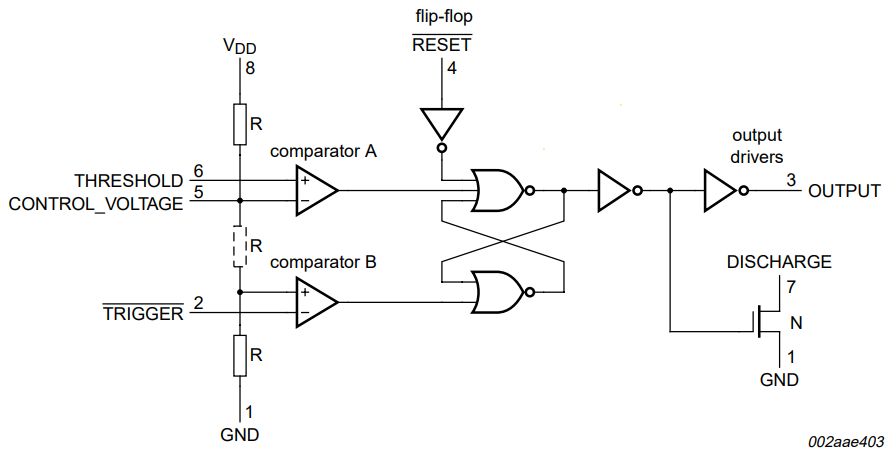
\includegraphics[width=1\linewidth]{images/ICM7555-functional-diagram.png}
	\caption{The functional diagram, where pin 5 (CONTROL\_VOLTAGE) and the positive terminal of comparator B represent ${\mbox{2/3V}}_{\mbox{DD}}$ and ${\mbox{1/3V}}_{\mbox{DD}}$, respectively.}
	\label{fig1}
\end{figure}
\begin{figure}[H]
	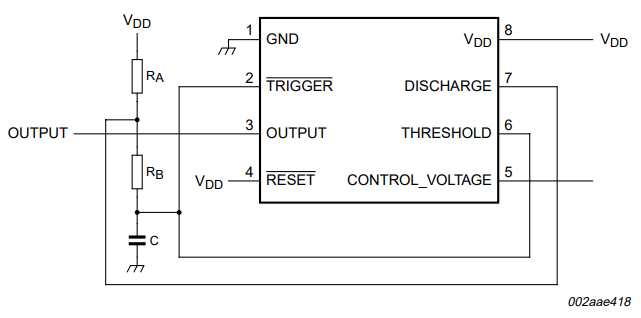
\includegraphics[width=1\linewidth]{images/ICM7555-astable-config.png}
	\caption{The astable configuration, where the voltage on capacitor C acts as a set and reset for the SR latch through both comparators.}
	\label{fig2}
\end{figure}

\noindent
The data sheet provides the frequency $f$ and duty cycle $\delta$ of the square wave output, given the values of ${\mbox{R}}_{\mbox{A}}$, ${\mbox{R}}_{\mbox{B}}$, and C:
\begin{align*}
f &= \dfrac{1.44}{(R_A+R_B)\times{C}}
\\
\delta &= \frac{R_{A}+R_{B}}{R_{A}+2R_{B}}
\end{align*}

\noindent
For the frequency, the resistors and capacitor are inversely proportional to the frequency as the time constant is increased. The duty cycle is solely dependent on the ratio of both resistors. Theoretically, according to the given resistor values in Figure \ref{fig4}, f $\simeq$ 1.53Hz and $\delta \simeq$ 50\%.

\begin{figure}[H]
	\centering
	
\includegraphics[width=0.7\linewidth]{images/astable-waveform.png}
	\caption{The waveform of the astable configuration.}
	\label{fig3}
\end{figure}

\subsection{Schematic}

\begin{figure}[H]
	\centering
	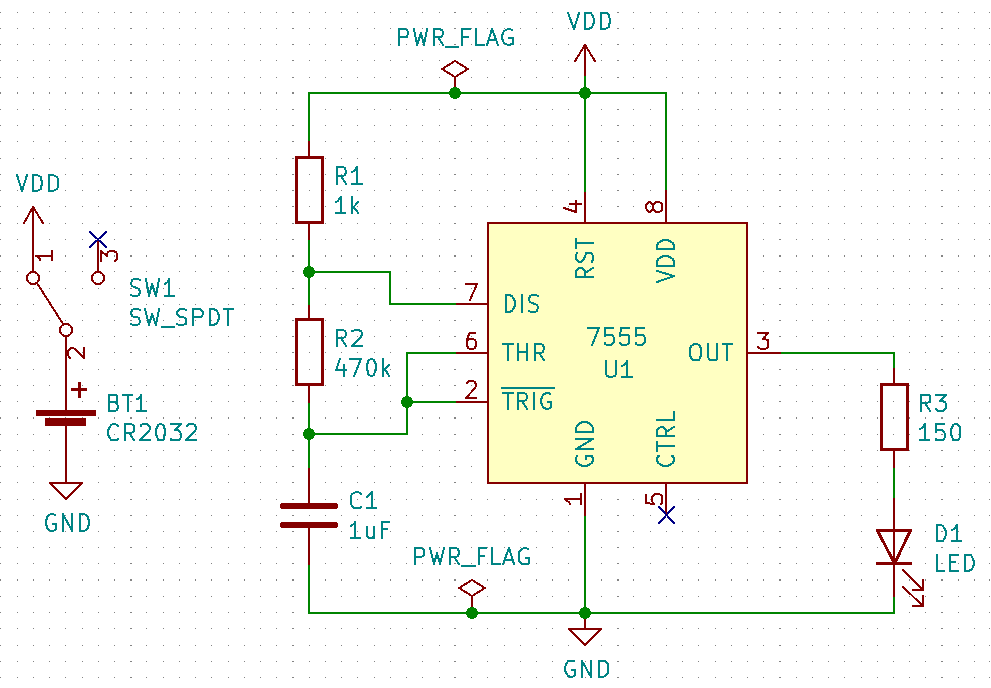
\includegraphics[width=1\linewidth]{images/schematic.png}
	\caption{The schematic of the circuit in KiCad.}
	\label{fig4}
\end{figure}

%BOM - unnecessary
\begin{comment}
\begin{table}[H]
	\small
	\begin{tabular}{c|l|l}
	\hline
	Index & Schematic Part Number & Manufacturer Part Number \\ \hline
	1	  & R1					  & RC1206FR-071KL \\
	2	  & R2					  & RC1206FR-07470KL \\
	3	  & C1					  & CL31A105KB9LNNC \\
	4	  & D1					  & APT3216LVBC/D \\
	5	  & R3					  & RC1206FR-07100RL \\
	6	  & CR2032				  & 3034 \\
	7	  & U1					  & ICM7555IBAZ-T \\
	8	  & SW1					  & JS102011SCQN \\
	\hline
	\end{tabular}
	\caption{BOM (Bill of Materials)}
	\label{table1}
\end{table}
\end{comment}

\subsection{Design}

\begin{figure}[H]
\centering
\begin{subfigure}{0.45\linewidth}
  \centering
  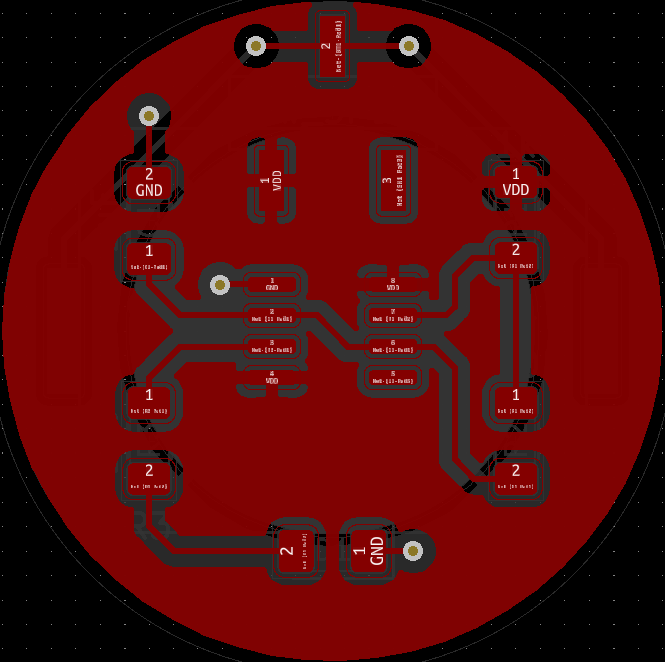
\includegraphics[width=1\linewidth]{images/PCB-front.png}
  \caption{The front copper layer}
  \label{fig5sub1}
\end{subfigure}
\begin{subfigure}{0.45\linewidth}
  \centering
  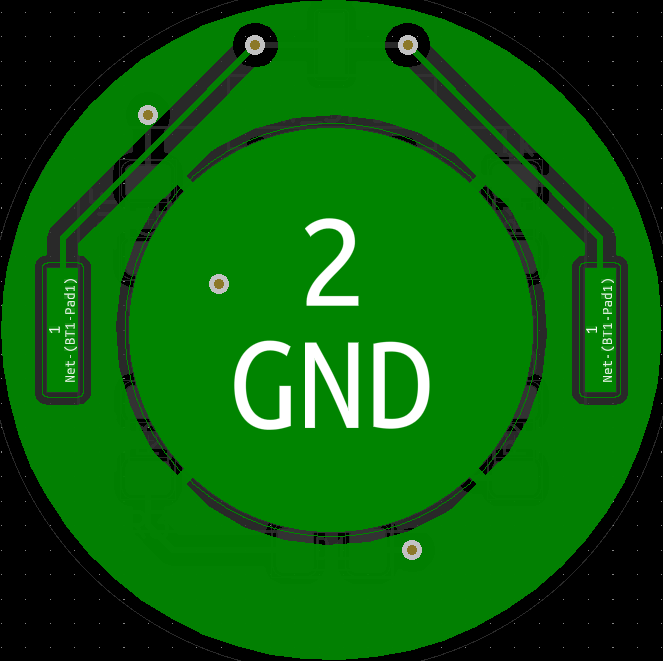
\includegraphics[width=1\linewidth]{images/PCB-back.png}
  \caption{The back copper layer}
  \label{fig5sub2}
\end{subfigure}
\caption{The PCB design}
\label{fig:test}
\end{figure}
\noindent
For the PCB design, the 7555 timer was placed exactly in the middle of the circular cut-out. A circular shape was chosen to fit the contour of the 2032 cell battery, and both the top and bottom layers were plated with a power and ground plane, respectively.

\section{Summary}

% Actual frequency on Oscilloscope, soldered board
\subsection{Results}

\subsection{What was Learned}
\begin{compactitem}
  \item Basic PCB structure.
  \item Creating custom footprints via a data sheet.
  \item Creating custom symbols for chips.
  \item PCB layout and design in KiCad.
  \item Trace width and other sizing constraints.
\end{compactitem}

\subsection{Sources}
\begin{compactitem}
  \item \url{https://en.wikipedia.org/wiki/555_timer_IC}
  \item \url{https://www.renesas.com/us/en/document/dst/icm7555-icm7556-datasheet}
  \item \url{https://www.youtube.com/c/contextualelectronics}
\end{compactitem}

\end{document}
